% Options for packages loaded elsewhere
\PassOptionsToPackage{unicode}{hyperref}
\PassOptionsToPackage{hyphens}{url}
%
\documentclass[
]{article}
\usepackage{lmodern}
\usepackage{amsmath}
\usepackage{ifxetex,ifluatex}
\ifnum 0\ifxetex 1\fi\ifluatex 1\fi=0 % if pdftex
  \usepackage[T1]{fontenc}
  \usepackage[utf8]{inputenc}
  \usepackage{textcomp} % provide euro and other symbols
  \usepackage{amssymb}
\else % if luatex or xetex
  \usepackage{unicode-math}
  \defaultfontfeatures{Scale=MatchLowercase}
  \defaultfontfeatures[\rmfamily]{Ligatures=TeX,Scale=1}
\fi
% Use upquote if available, for straight quotes in verbatim environments
\IfFileExists{upquote.sty}{\usepackage{upquote}}{}
\IfFileExists{microtype.sty}{% use microtype if available
  \usepackage[]{microtype}
  \UseMicrotypeSet[protrusion]{basicmath} % disable protrusion for tt fonts
}{}
\makeatletter
\@ifundefined{KOMAClassName}{% if non-KOMA class
  \IfFileExists{parskip.sty}{%
    \usepackage{parskip}
  }{% else
    \setlength{\parindent}{0pt}
    \setlength{\parskip}{6pt plus 2pt minus 1pt}}
}{% if KOMA class
  \KOMAoptions{parskip=half}}
\makeatother
\usepackage{xcolor}
\IfFileExists{xurl.sty}{\usepackage{xurl}}{} % add URL line breaks if available
\IfFileExists{bookmark.sty}{\usepackage{bookmark}}{\usepackage{hyperref}}
\hypersetup{
  pdftitle={Maintainance of Certification and Medicare Outcomes},
  pdfauthor={Xilin Chen},
  hidelinks,
  pdfcreator={LaTeX via pandoc}}
\urlstyle{same} % disable monospaced font for URLs
\usepackage[margin=1in]{geometry}
\usepackage{graphicx}
\makeatletter
\def\maxwidth{\ifdim\Gin@nat@width>\linewidth\linewidth\else\Gin@nat@width\fi}
\def\maxheight{\ifdim\Gin@nat@height>\textheight\textheight\else\Gin@nat@height\fi}
\makeatother
% Scale images if necessary, so that they will not overflow the page
% margins by default, and it is still possible to overwrite the defaults
% using explicit options in \includegraphics[width, height, ...]{}
\setkeys{Gin}{width=\maxwidth,height=\maxheight,keepaspectratio}
% Set default figure placement to htbp
\makeatletter
\def\fps@figure{htbp}
\makeatother
\setlength{\emergencystretch}{3em} % prevent overfull lines
\providecommand{\tightlist}{%
  \setlength{\itemsep}{0pt}\setlength{\parskip}{0pt}}
\setcounter{secnumdepth}{-\maxdimen} % remove section numbering
\usepackage{booktabs}
\usepackage{longtable}
\usepackage{array}
\usepackage{multirow}
\usepackage{wrapfig}
\usepackage{float}
\usepackage{colortbl}
\usepackage{pdflscape}
\usepackage{tabu}
\usepackage{threeparttable}
\usepackage{threeparttablex}
\usepackage[normalem]{ulem}
\usepackage{makecell}
\usepackage{xcolor}
\ifluatex
  \usepackage{selnolig}  % disable illegal ligatures
\fi

\title{Maintainance of Certification and Medicare Outcomes}
\usepackage{etoolbox}
\makeatletter
\providecommand{\subtitle}[1]{% add subtitle to \maketitle
  \apptocmd{\@title}{\par {\large #1 \par}}{}{}
}
\makeatother
\subtitle{Cohort Definition}
\author{Xilin Chen}
\date{2021-04-19}

\begin{document}
\maketitle

{
\setcounter{tocdepth}{3}
\tableofcontents
}
This document describes how the ABS maintance of certification and
medicare outcomes cohort was defined. The data will be used for further
statistical analyses.

\hypertarget{data-sources}{%
\subsection{1. Data Sources}\label{data-sources}}

\begin{itemize}
\tightlist
\item
  ABS certification data (recerived at September 2019 from ABS)
\item
  Medicare claim data

  \begin{itemize}
  \tightlist
  \item
    Year: 2007-2018
  \item
    Procedures: commonly performed general surgery procedures (162
    procedures in total)
  \end{itemize}
\end{itemize}

ABS and Medicare claim data are linked using phycisian NPIs.

\hypertarget{data-process}{%
\subsection{2. Data Process}\label{data-process}}

\hypertarget{abs}{%
\subsubsection{ABS}\label{abs}}

\hypertarget{inclusion-and-exclusion}{%
\subsubsection{1. Inclusion and
Exclusion}\label{inclusion-and-exclusion}}

Inclusion:

\begin{itemize}
\tightlist
\item
  Surgeons with NPI
\item
  Passed initial certification exam
\end{itemize}

Exclusion:

\begin{itemize}
\tightlist
\item
  Fellowship or non-US trained surgeons (n = 14523).

  \begin{itemize}
  \tightlist
  \item
    Fellowship and Med school information is from ABS, AMA and
    Fellowship Council data.
  \end{itemize}
\end{itemize}

Below is the re-certification status for all qualified ABS surgeons.
Very few surgeons have recorded failed re-certification status. A large
portion of surgeons didn't have re-certification records at all,
i.e.~NA.

\begin{table}[H]
\centering
\begin{tabular}{r|r|l}
\hline
ReCeverPassed & n suregon & percentage\\
\hline
0 & 154 & 0.5\%\\
\hline
1 & 16532 & 53.2\%\\
\hline
NA & 14380 & 46.3\%\\
\hline
\end{tabular}
\end{table}

\hypertarget{define-never-recertified-surgeon-group-define-na-group}{%
\subsubsection{2. Define never recertified surgeon group (Define NA
group)}\label{define-never-recertified-surgeon-group-define-na-group}}

\hypertarget{at-least-have-10-years-after-the-initial-certification-year}{%
\paragraph{2.1. At least have 10 years after the initial certification
year}\label{at-least-have-10-years-after-the-initial-certification-year}}

The ABS require diplomats certified subsequently to pass a secure,
multiple-choice comprehensive recertification examination in surgery
every 10 years.

4522 surgeons who had no recertification record but had initial board
certification more than 10 years ago. We include this group as failed
recertification group. Surgeons who didn't have 10 years after the
initial certification process were excluded because they didn't have
enough time to pass the re-certification exam.

\hypertarget{grandfathered-out-of-the-recertification-process}{%
\paragraph{2.2 Grandfathered out of the recertification
process}\label{grandfathered-out-of-the-recertification-process}}

We excluded surgeons who had their initial certification before 1976. It
was bases on the recertification was introduced at 1976 ``the American
Board of Surgery (ABS) introduced time-limited certification in 1976,
requiring diplomats certified subsequently to pass\ldots{}''. If the
surgeon was initially certified before 1976, she/he was not required for
recertification at the initial certification time.

242 surgeons graduated before 1976 and are excluded in the analyses
cohort.

\begin{table}[H]
\centering
\begin{tabular}{l|r|l}
\hline
Recert\_status & n suregon & percentage\\
\hline
failed & 154 & 1\%\\
\hline
NA\_failed & 4280 & 20\%\\
\hline
passed & 16532 & 79\%\\
\hline
\end{tabular}
\end{table}

\hypertarget{data-linkage}{%
\subsection{3. Data linkage}\label{data-linkage}}

\begin{itemize}
\tightlist
\item
  Only keep cases that performed 10 years after initial certification.

  \begin{itemize}
  \tightlist
  \item
    The ABS gives 10 years for surgeons for the recertification. We keep
    cases that 10 years after the initial certification to better
    capture the impact of the recertification process.
  \end{itemize}
\end{itemize}

Link ABS with Medicare by NPI. Below is the number of surgeons by each
recertification category after linked with Medicare outcomes.

\begin{table}[H]
\centering
\begin{tabular}{l|r|l}
\hline
Recert\_status & n suregon & percentage\\
\hline
failed & 62 & 0\%\\
\hline
NA\_failed & 1827 & 12\%\\
\hline
passed & 13011 & 87\%\\
\hline
\end{tabular}
\end{table}

6066 (29\%) surgeons from ABS didn't have recorded medicare outcomes.

\hypertarget{cohort-definition-diagram}{%
\subsection{4. Cohort definition
diagram}\label{cohort-definition-diagram}}

Below is the consort diagram for the data selection process

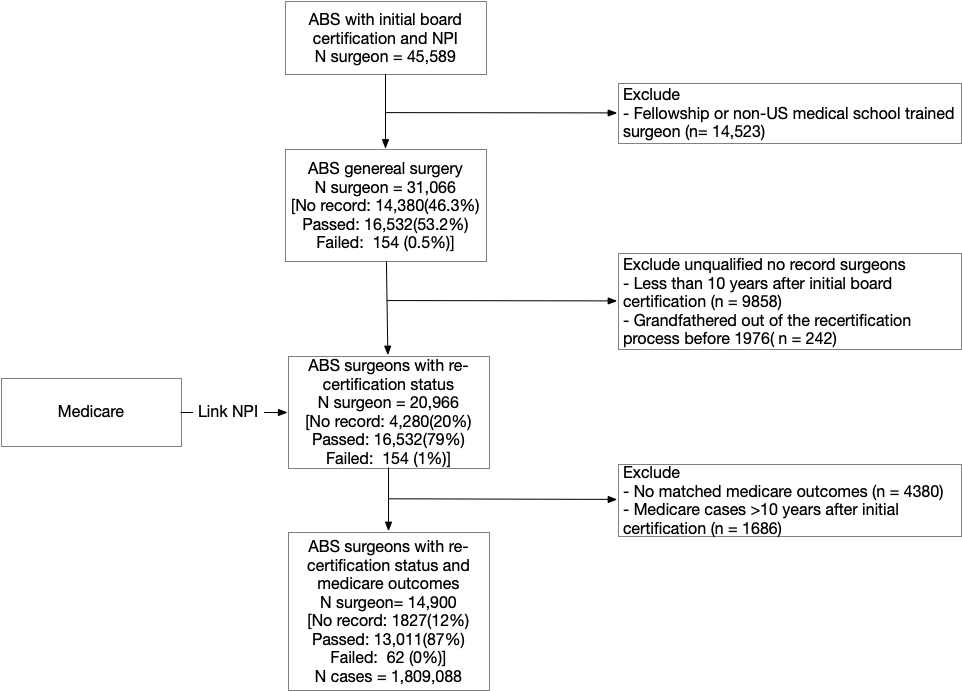
\includegraphics{/Users/xilinchen/Documents/Repo/ABS_MoC_vs_pt_Outcome/other_docs/Diagram/cohort_definition/cohort_definition.png}

\end{document}
